\chapter{Introduction}
As an introduction to the work that was done during this thesis, this chapter starts with presenting a brief overview on the relevance of quantum computing, and describing the motivation behind this work.
After that, the objective of this work is described and an outline of this report is given.

\section{Motivation}
Quantum computing is a new model of computation that promises to solve certain problems more efficiently than classical computers by making use of quantum mechanical phenomena such as superposition and interference.
The idea of quantum computing originated from~\textcite{benioff1980computer}, who proposed a quantum mechanical model of the Turing machine in 1980.
This idea was later extended as \textcite{manin1980vychislimoe} and \textcite{feynman1982simulating} independently suggested that quantum computers have the potential to solve certain computational problems intractable by classical computers.
Since then, researchers have been searching for applications for quantum computing.
Some noteworthy developments in the field of quantum computing include Shor's algorithm for factoring integers~\cite{shor1999polynomial} and Grover's algorithm for unstructured database search~\cite{grover1996fast}.
These quantum algorithms promise an exponential and quadratic speedup respectively over their best-known classical counterparts.
The finding of such speedups have catalyzed research towards quantum computers, and more applications have since been found in fields including chemistry~\cite{mcardle2018quantum}, cryptography~\cite{bennett2014quantum}, and machine learning~\cite{biamonte2017quantum}.

Until recently, quantum computing had been a mainly theoretical field.
These days, however, thanks to recent technological advances, various quantum devices are being actively developed.
Furthermore, technological giants such as IBM, Microsoft, Intel, and Google are investing heavily in the development of quantum computers.
The applications of these current quantum devices are very limited however, due to their inability to store information for a long time and their sensitivity to errors.
For instance, \textcite[Appendix~M]{fowler2012surface} estimate that to factor a 2000-bit number using Shor's algorithm would require a quantum computer with about a billion physical qubits, and error rates below $4 \times 10^{-13}$.
In contrast, devices today have about 50 to 100 physical qubits and error rates above $0.1$.

These small and error-prone quantum devices, referred to as \gls{nisq} devices, may be unfit to run quantum algorithms like Shor's algorithm, but they may still prove to be useful and perform tasks intractable by classical computers~\cite{preskill2018quantum}.
To deal with the limitations of \gls{nisq} devices, \glspl{hqca} are being actively researched.
These \glspl{hqca} combine classical and quantum computations as visualized in~\Cref{fig:hybrid-quantum-classical}.
\begin{figure}[ht]
    \centering
    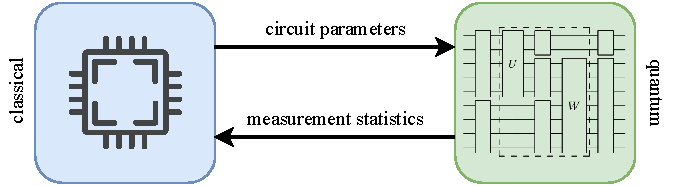
\includegraphics[width=0.65\linewidth]{figures/hybrid-quantum-algorithm.pdf}
    \captionof{figure}[General structure of a hybrid quantum-classical algorithm.]{General structure of a hybrid quantum-classical algorithm. The data interchange between the classical and quantum part is often repeated many times.}
    \label{fig:hybrid-quantum-classical}
\end{figure}
\Acrlongpl{hqca} typically involve a small quantum computation inside of a classical optimization loop, greatly reducing the amount of quantum resources needed.
This makes them suitable to run on \gls{nisq} devices, and are expected to be one of the first useful applications for quantum computing~\cite{endo2021hybrid}.
It is important to note that \gls{nisq} devices running \glspl{hqca} will likely not be revolutionary by itself.
Instead, it should be seen as an important stepping stone towards more powerful quantum devices and algorithms.

Research towards \glspl{hqca} often involves executing quantum circuits on actual quantum chips or through quantum circuit simulation.
To support this kind of research, classical and quantum computing facilities are needed.
Furthermore, these facilities need to be connected and able to interchange data in a timely manner for this kind of research to be feasible.
This is especially challenging given that both quantum and classical resources are shared with other users.


\section{Objective}
The purpose of this thesis is to propose an infrastructure for the efficient execution of \acrlongpl{hqca}.
This work is in collaboration with TNO, QuTech, and SURF, and is focused on the efficient execution of \glspl{hqca} using QuTech's quantum computing platform Quantum Inspire~\cite{last2020quantum} and SURF's \gls{hpc} center.
To allow for the efficient execution of \glspl{hqca}, the SURF \gls{hpc} and Quantum Inspire job schedulers should be synchronized to minimize the execution of the algorithm.
A key part in this is figuring out sources of overhead and current bottlenecks.
In a hybrid setup like this, overheads such as quantum and classic scheduling wait times, data transfers, and resource initialization can quickly increase the run time of \glspl{hqca}.
%Quantum Inspire is a quantum computing platform that QuTech launched last year to make quantum systems available to the general public for exploratory research.
% TODO: how will we do this? benchmarking, bottlenecks, etc.

%Currently, there are four ways to run quantum computations using Quantum Inspire: running the QX quantum computer simulator on local resources, using Quantum Inspire's QX-26 simulator running on their commodity server, using the QX-31 simulator running on SURF's infrastructure, or using QuTech's Spin-2 or Starmon-5 \gls{qpu}.


\section{Outline}
This report is structured as follows. \Cref{chap:background} provides the reader with a background on computational complexity, quantum information, and quantum computation. \Cref{chap:hybrid-quantum-classical-algorithms} takes a deeper look into well-known \glspl{hqca} and their working.